%% LaTeX2e class for student theses
%% sections/content.tex
%% 
%% Karlsruhe Institute of Technology
%% Institute for Program Structures and Data Organization
%% Chair for Software Design and Quality (SDQ)
%%
%% Dr.-Ing. Erik Burger
%% burger@kit.edu
%%
%% Version 1.3.2, 2017-08-01


\chapter{An Approach for Adaptive Monitoring for Continuous Performance Model Integration}
\label{ch:An Approach for Adaptive Monitoring for Continuous Performance Model Integration}
In this chapter, we will introduce our approach for adaptive monitoring for continuous performance model integration. 

\section{Context of our approach}
\label{sec: Context of our approach}
As mentioned before, our approach is part of the CIPM vision (section 8) which extends the agile and DevOps process and provides them with iterative and incremental Performance Model. Moreover, the Performance Models in CIPM are enriched with Performance Model Parameters. In the following, we will briefly depict and describe the process and the context in which our approach takes place.\\

Figure \ref{fig:Context of our approach} shows the process in which our approach takes place. this process is based on Vitruvius (section 2) which means its elements are either models or transformations. The Java code in \ref{fig:Context of our approach} is represented by a JaMoPP model. When the developer commits changes on this model, two transformations will be triggered. The first one is the Coevolution process of Langhammer (section 5) which keeps the Source Code and the models in the Palladio Component Model consistent, mainly the repository and the SEFF Model. The second Transformation is our Transformation which is specified for keeping the Source Code and the Instrumentation Model consistent. We proposed the Instrumentation Model in order to persist the Probes that will be required for instrumenting the Source Code.\\

When the system under development is deployed, our Instrumentation Process will be triggered. This process receives as inputs the Probes from the Instrumentation Model and the Source Code of the System. It delivers afterwards the instrumented Source Code as a JaMoPP Model. After the instrumentation process has been finished, the instrumented Source code will be executed and monitored.  The information provided by monitoring are encapsulated in a Measurement Model which describes the needed monitoring records.  After the monitoring has been finished the Parameters Estimation Process (section 9) will be triggered. it uses the information in the Measurement Model to estimate the Performance Model Parameters and updates accordingly the SEFF Model in the Palladio Component Model. Afterwards, the user can use the updated Performance Model to simulate and evaluate the performance of the system. \\


\begin{figure}[h]
\centering
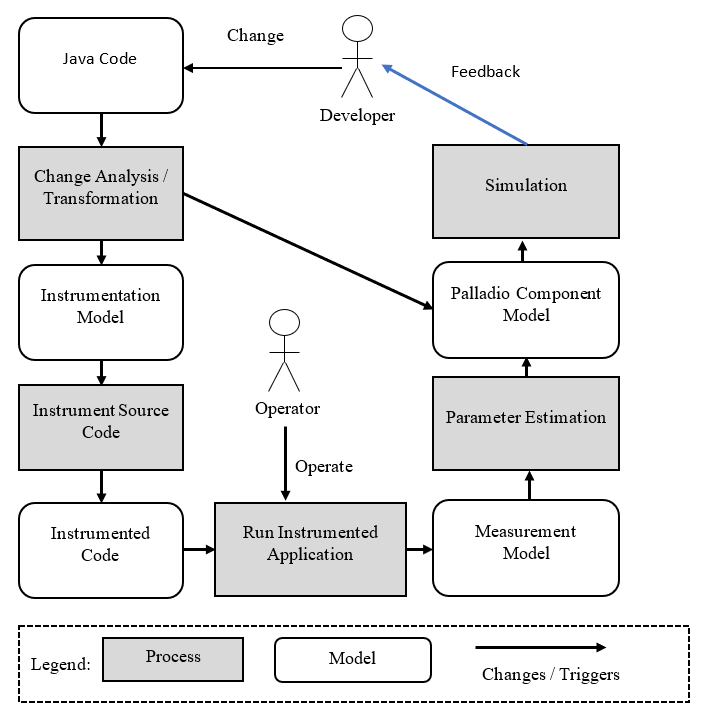
\includegraphics[width=0.9\textwidth]{figures/approach_context}
\caption{Context of our approach}
\label{fig:Context of our approach}
\end{figure}


\section{Monitoring Probes}
\label{sec:Monitoring Probes}
Monitoring Probes are responsible for collecting monitoring information from the system. Furthermore, they can be specified based on the needed monitoring information. For example, if we need to monitor the response time of a service and the number of execution of loops, we can specify two monitoring probes, one probe for the response time and the other for loops execution number. \\

In our approach, we want to provide monitoring information for Palladio Performance Model which are described in terms of SEFF (section 1.2).   SEFF Model is composed from four main elements which inherit from the so-called Abstract Action, namely Internal Action, Branch Action, Loop Action and Service Call Action. In other words, we should specify probes that provide these elements with the needed monitoring information. Therefore, we defined a monitoring probe for each SEFF element Figure 2. The monitoring information that we need to produce for SEFF elements are described in (section 1.3) under monitoring records.  \\

For the monitoring purpose, we used the Kieker Monitoring Framework (section 6) which offers the possibility to define new monitoring probes based on the needed monitoring records.\\

\begin{figure}[h]
\centering
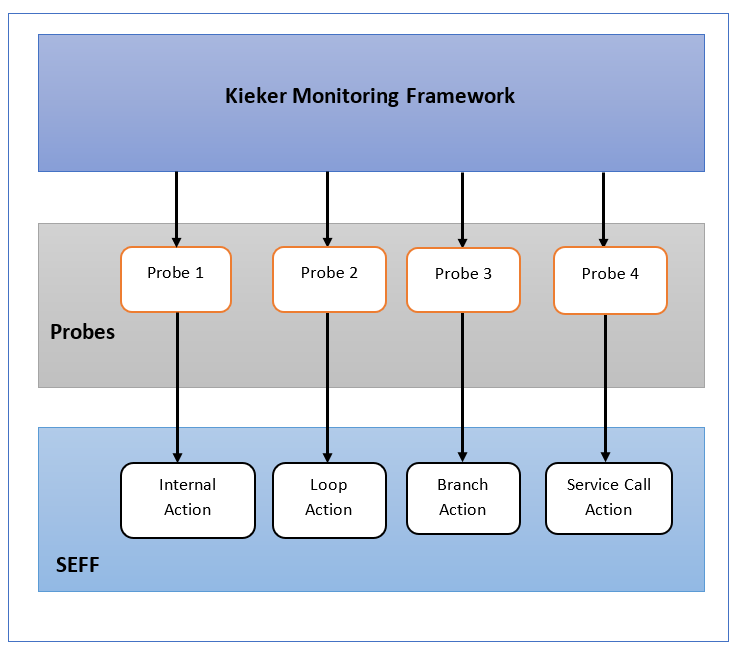
\includegraphics[width=0.9\textwidth]{figures/probes}
\caption{Specified Monitoring Probes in our Approach}
\label{fig:Specified Monitoring Probes in our Approach}
\end{figure}

\section{Monitoring Records}
\label{sec:Monitoring Records}
In order to create monitoring probes (section 1.2), one must define first of all   the needed monitoring information. in our case, we defined monitoring probes for SEFF model which are based on the monitoring records in Figure 3. \\

Figure 3 shows an UML Class Diagram that describe the monitoring records. It provides extra information that are needed for the purpose of performance model parameters estimations. The abstract class RecordWithSession specifies a sessionID attribute that helps to identify the monitoring information based on sessions.  The abstract class ServiceContextRecord adds a serviceExecutionID attribute that helps to reference a ServiceCallRecord.\\

All records are identified via their ids. The id of each record can be provided by the used monitoring framework. However, in order to be able to use these records for SEFF models we’ve used for each record the id of the corresponding SEFF element. \\

For internal actions which express internal computation, we want to know the time consumed by them. Therefore, we need to log the id of the internal action, start time and stop time. \\

For Loops, we need to recognize the number of executions of a loop. The same thing for branches, we log the id of the executed branch in order to realise if the branch was executed or not. \\

As to service calls, we need to locate them in which service are called, we need also to provide the response time and the parameters they are given. The parameters of services are given in a JSON format.\\

\begin{figure}[h]
\centering
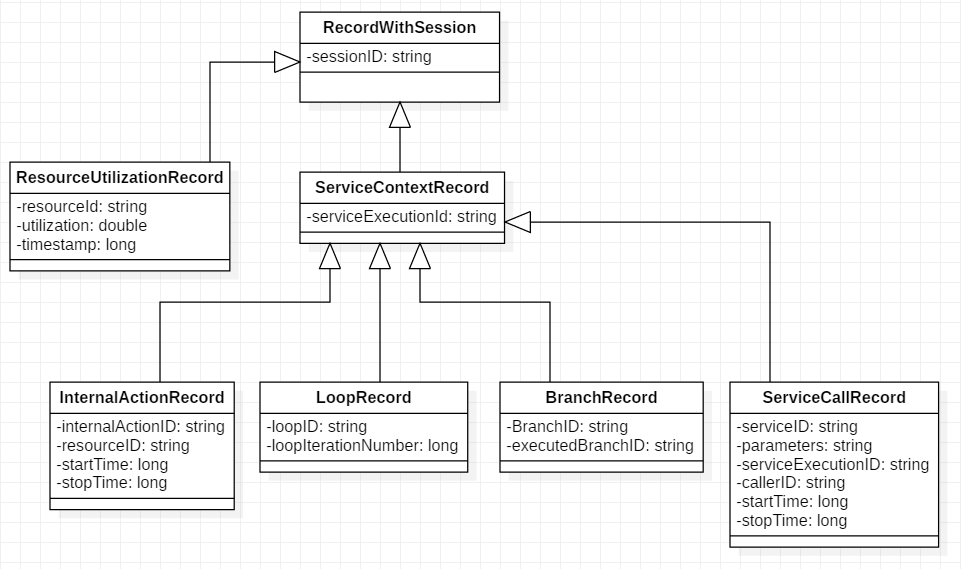
\includegraphics[width=0.9\textwidth]{figures/records}
\caption{UML class diagram that shows the monitoring information required by SEFF models}
\label{fig:records}
\end{figure}

\section{Adaptive Instrumentation}
\label{sec:Adaptive Instrumentation}
In this section, we will introduce the meaning of Adaptive Monitoring in our approach as well as the main concepts used in order to achieve that.\\

As mentioned before, our approach is addressed to iterative development processes like DevOps. In this context, Adaptive Instrumentation means that only the parts of the source code that have been changed in the current iteration will be monitored. \\

Based on this definition, we should be able to generate instrumentation points during the development phase. In order to do this, we decided to use two main concepts which are model-driven engineering and change-driven engineering. Moreover, our approach is based on the Coevolution approach which itself uses these two concepts to keep the source code and the architecture models consistent. Precisely, the Coevolution approach uses change-driven consistency preservation in order to keep the Java source code and SEFF models consistent. Changes in the source code model are monitored and transformed to changes in the SEFF model based on defined consistency-preservation rules. \\

In order to achieve an adaptive instrumentation in our approach, we’ve defined and Instrumentation Model which contains the instrumentation points. Moreover, we defined a transformation that monitored changes in the source code model and creates the corresponding instrumentation points in the instrumentation model. \\

In order to keep the source code and the instrumentation model consistent, we've used Vitruvius Framework which makes it possible to keep models instances consistent based on models changes. 

\section{Adaptive Monitoring}
\label{sec:Adaptive Monitoring}
Adaptive Monitoring means that the monitoring probes can be activated and deactivated based on the existing monitoring information. this is needed when we’ve collected enough monitoring information for some probes but they still can log monitoring information which is not needed and which can lead to monitoring and performance model parameters estimations overhead.  Therefore, adaptive monitoring can help to reduce the monitoring overhead by reducing the number of monitoring probes. \\

In order to achieve Adaptive Monitoring in our approach, we’ve added an attribute for the monitoring probes that defines their activeness. That means, monitoring probes are checked during the monitoring phase and they can log monitoring information only if the are activated. The deactivation of the probes can be done for example, when we've realised that the current monitoring information for these probes are enough for the performance model parameters estimation.\\

\section{Instrumentation Model}
\label{sec:Instrumentation Model}
The Instrumentation Model was originally presented in the approach of Manar and Koziolek \cite{mazkatli2018continuous} on which we based our approach. 

The Instrumentation Model (IM) Figure \ref{fig:im} is one of the Contribution of this thesis in Vitruvius. IM is responsible for describing and managing the instrumentation points. Moreover, we've defined IM in order to achieve the Adaptive Instrumentation (Section \ref{sec:Adaptive Instrumentation}) and Adaptive Monitoring (Section \ref{sec:Adaptive Monitoring}).\\

IM is composed from two elements, AppProbes which represents the model root and the element Probe which represents an instrumentation point. The element Probe corresponds to a SEFF abstract action which can be an Internal Action, a Branch Action, a Loop Action or a Service Call Action.\\

As mentioned before, we’ve used Vitruvius in order to keep the source code and the IM consistent. We've also extended the Coevolution approach which uses also Vitruvius to keep the Java source code and the architecture models consistent. The Coevolution approach uses an instance of the SEFF model in which our probes are stored. Therefore, in order to avoid redundant information within Vitruvius, we've decided to store only the Ids of these probes which give us the possibility to return them when they are needed. Moreover, since the probes represent concretely the four above mentioned abstract actions of SEFF, the id of a probes is named abstractActionID. Furthermore, we've added a boolean attribute to the monitoring probes in order to enable to adaptive monitoring. \\

\begin{figure}[h]
\centering
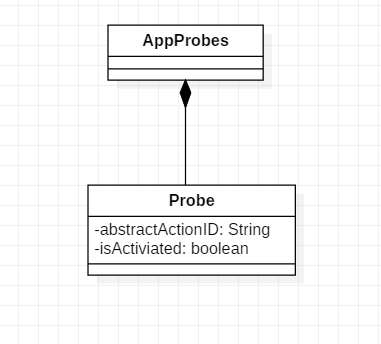
\includegraphics[width=0.5\textwidth]{figures/im}
\caption{UML Class Diagram that represents the Instrumentation Model}
\label{fig:im}
\end{figure}


\section{Approach}
\label{sec:approach}
In this section we will briefly introduce our approach as well as the context in which our activities will be executed. Further details on these activities will be presented in the next chapters.\\

our approach is developed in the context of the iterative development process DevOps. Therefore, Figure \ref{fig:devops_approach} gives an overview of the activities of our approach and in which DevOps phase they can be executed. The green color indicates processes or model in which our algorithms are executed. \\

In our approach we've defined to main processes. The first one is responsible for collecting the instrumentation points or the probes. It must be executed during the development phase. It uses information from Vitruvius and it's based on the Coevolution approach. The Coevolution approach keeps the source code and the SEFF model consistent and provides us with information that help to gather the probes. Vitruvius is used to keep the source code model and the Instrumentation Model consistent. The generated probes are saved and managed in the Instrumentation Model. For more details on the probes generation process, look at the chapter (Probes Generation Process).\\

The second process is the instrumentation process which can be executed at any time. Once it's executed, it takes the probes from the Instrumentation Model and insert the instrumentation source code in the source code of the system based on the types of the probes (Figure 2). However, if the monitoring will be firstly done in the monitoring phase of DevOps, this process can be automatically triggered at the Continuous Deployment phase. For more details on our instrumentation process look at the chapter (Source Code Instrumentation Process).\\

In the monitoring phase, the instrumented system can be executed in order to log monitoring information. Moreover, in order to achieve an adaptive monitoring, the monitoring probes execute a self-checking for their activeness. Therefore, the monitoring code uses information from the Instrumentation Model in order to check if probes are activated of deactivated and thus if they can log or not. \\


\begin{figure}[h]
\centering
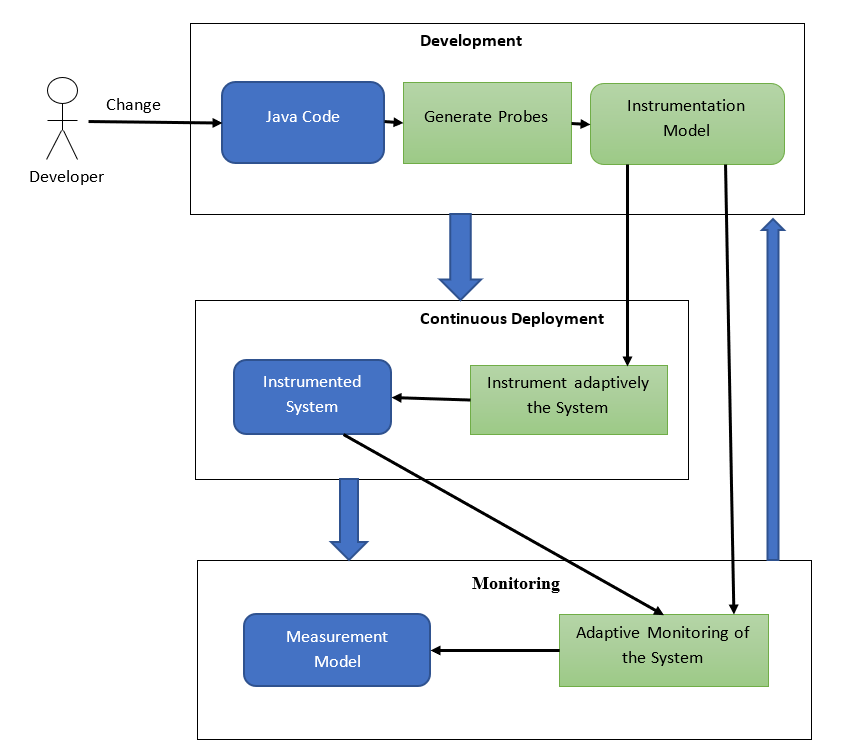
\includegraphics[width=0.9\textwidth]{figures/devops_approach}
\caption{Overview of our Approach Activities in DevOps context}
\label{fig:devops_approach}
\end{figure}




 